\subsection{The Higgs Boson}
\label{Intro_Higgs}

\begin{figure}[htb]
  \begin{center}
    {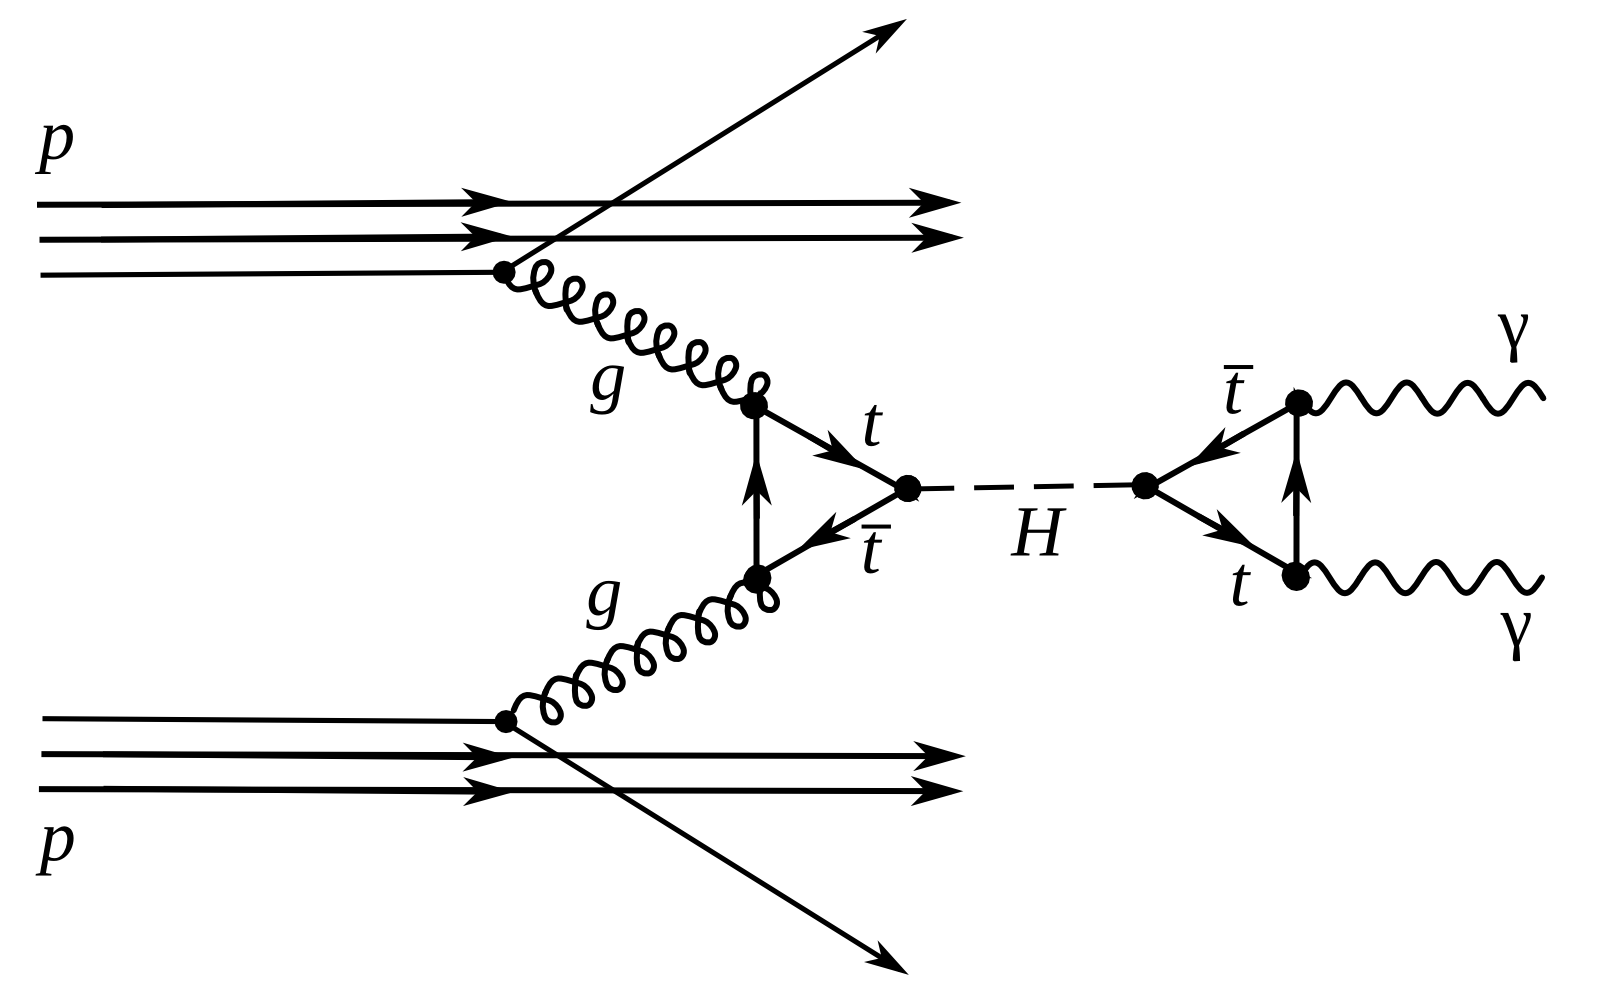
\includegraphics[width=0.80\textwidth]{../figs/Intro/higgsProduction.png}}
    \caption{Higgs production and decay}
    \label{fig:higgsProduction}
  \end{center}
\end{figure}

In combining the electromagnetic and the weak interactions there is a question why the photon is massless while W and Z bosons are massive and how to accommodate these masses in the Standard Model. It was proposed independently by three different groups of theorists in 1960s that these bosons are getting mass by interacting with a massive scalar field. The quant of this field is called the Higgs boson (following the name of one of the theorists) and the mechanism of W and Z boson to get mass is called the Higgs mechanism. 

At the descriptive level the mechanism can be explained in a way that a particle is born massless but while traveling through the Higgs field it is being slowed down and that is how is gets its inertia. In this understanding, it is intuitive that higher mass of a particle means stronger interaction with the Higgs field. 

Although the Higgs mechanism was introduced to accommodate masses of W$^\pm$ and Z bosons only, the same approach can be used to introduced masses of all elementary particles.

For many years the Higgs boson was the only missing particle in the Standard Model however in 2012 it was discovered by ATLAS and CMS collaborations in the reaction shown in Fig. \ref{fig:higgsProduction} in $\gamma\gamma$ and ZZ decay channels. 

The Feynman diagram with the dominant process of the Higgs production and its further decay to $\gamma\gamma$ is shown in Fig.\ref{fig:higgsProduction} where the Higgs is produced in the process of the gluon-gluon fusion through the top quark loop. The Higgs boson can be produced through any quark loop however a top quark is much more massive than any other quark and therefore has a much higher probability to produce a Higgs boson. 

The discovery of the Higgs boson is one of the most important scientific results in the past few years (alongside with the direct detection of the gravitational waves). Two of the theorists who proposed the Higgs mechanism, Francois Englert and Peter Higgs, were awarded the Nobel Prize in Physics in 2013.


